\documentclass{beamer}
\hypersetup{
    colorlinks=true,
    linkcolor=blue,
    filecolor=magenta,      
    urlcolor=cyan,
    pdftitle={Overleaf Example},
    pdfpagemode=FullScreen,
    }

\usepackage{caption}
\captionsetup{labelformat=empty, textfont=it}

% Chargement du logo
\logo{\includegraphics[height=0.75cm]{images/logo_enseirb.jpg}}

% Choix du thème
\usetheme{CambridgeUS}  % Thème de présentation
\usecolortheme{dolphin} % Thème de couleurs

% Informations sur la présentation
\title{Séance du 24/01}
\author{Projet S8: TRACK}
\institute[T2, Enseirb-Matmeca]{Département Télécommunication\\Enseirb-Matmeca, Bordeaux}
\date{\today}

% Début du document
\begin{document}

% Page de titre
\begin{frame}
  \titlepage
\end{frame}

% Introduction
\begin{frame}
  \frametitle{Ordre du Jour}
  \begin{itemize}
    \item Présentation des avancées
    \item Méthodes et Outils
    \item Présentation du calendrier
    \item Questions 
  \end{itemize}
\end{frame}

% Compte rendu des avancées
\begin{frame}
  \frametitle{Compte rendu des avancées}
  \begin{itemize}
    \item MRU :
    \begin{itemize}
        \item[\hspace{1cm}] Théorie implémentée sous Python
        \item[\hspace{1cm}] Premières trajectoires 
    \end{itemize}
    \item MUA et Singer
    \begin{itemize}
        \item[\hspace{1cm}] Calculs théoriques réalisés
        \item[\hspace{1cm}] Implémentation sous Python et génération de trajectoires
    \end{itemize}
    \item Création d'une bibliothèque de fonctions communes
    \begin{itemize}
        \item[\hspace{1cm}] Génération de coordonnées X et Y
        \item[\hspace{1cm}] Stockages des itérations de générations de vecteurs
        \item[\hspace{1cm}] Fonctions d'affichages des données
    \end{itemize}
  \end{itemize}
\end{frame}

% Graphiques Trajectoires
\begin{frame}
  \frametitle{Graphiques et Trajectoires : MRU}
  \hspace{1,7cm} $X$ \hspace{3cm} $Y$
  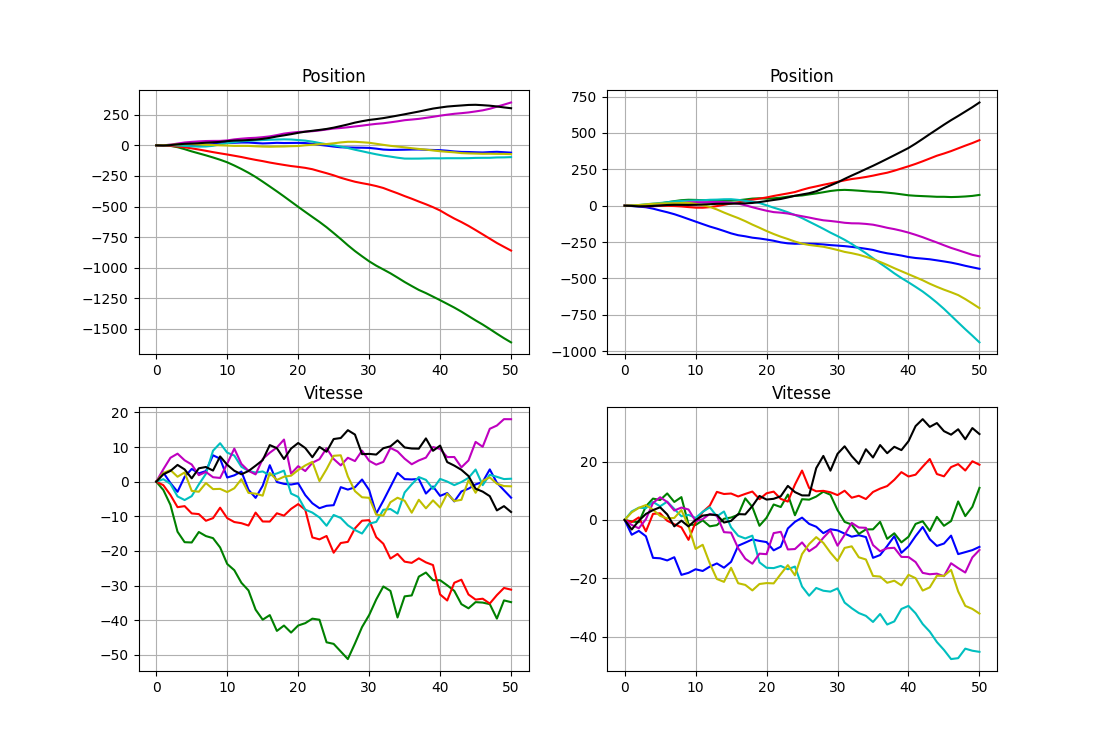
\includegraphics[width=.65\textwidth]{images/MRU_Générations.png}\hfill
  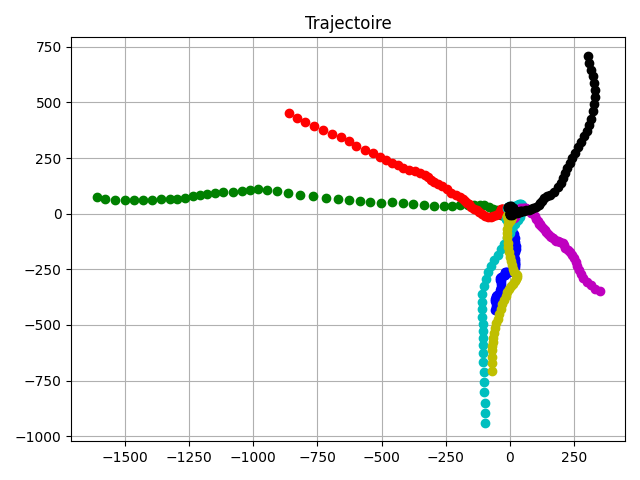
\includegraphics[width=.35\textwidth]{images/MRU_Trajectoires.png} 
  Paramètres : $T_{ech} = 1$, $N = 50$ et $\sigma^{2} = 3$
\end{frame}

\begin{frame}
  \frametitle{Graphiques : MUA}
  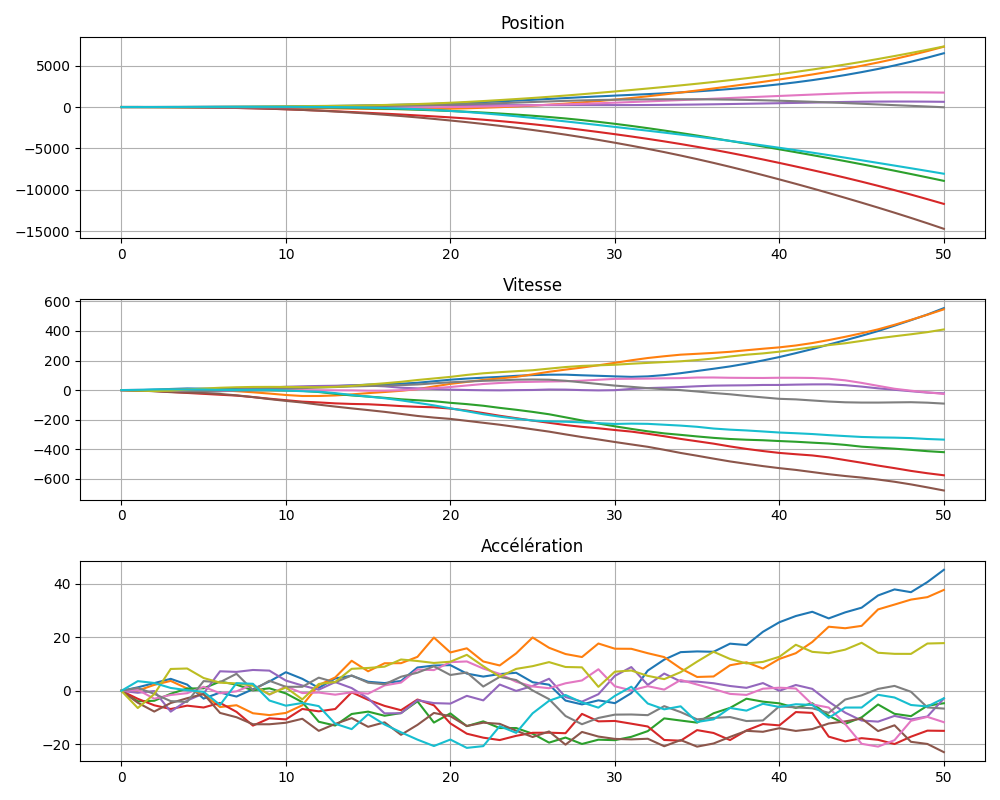
\includegraphics[width=0.75\textwidth]{images/MUA_Générations.png} \\
  Paramètres : $T_{ech} = 1$, $N = 50$ et $\sigma^{2} = 3$
\end{frame}

\begin{frame}
  \frametitle{Trajectoires : MUA}
  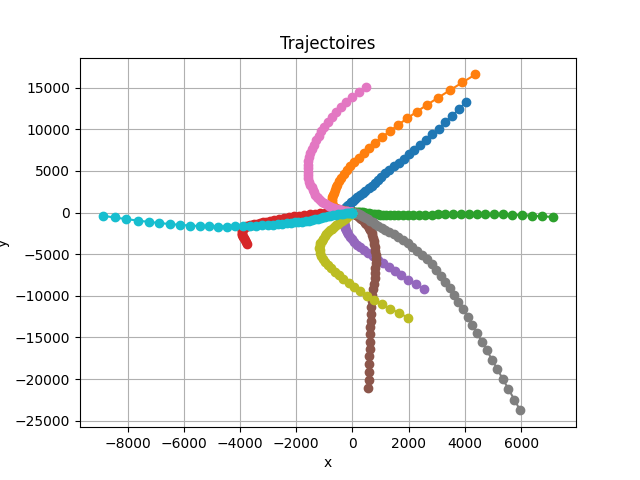
\includegraphics[width=0.75\textwidth]{images/MUA_Trajectoires.png} \\
  Paramètres : $T_{ech} = 1$, $N = 50$ et $\sigma^{2} = 3$
\end{frame}

\begin{frame}
  \frametitle{Graphiques et Trajectoires : Singer}
  \hspace{1,4cm} $X$ \hspace{2,5cm} $Y$ \\
  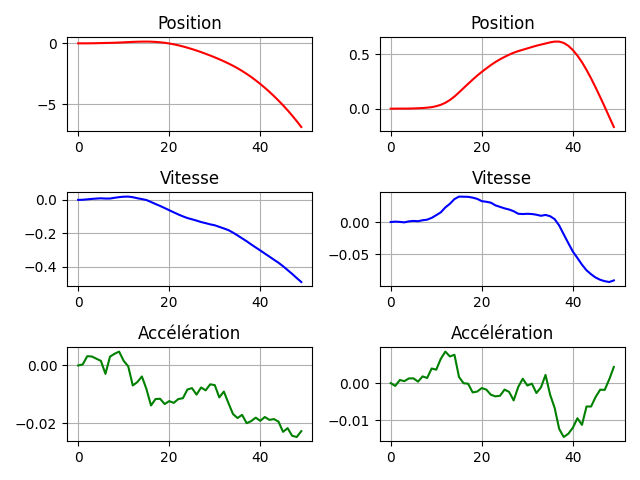
\includegraphics[width=.5\textwidth]{images/SINGER_Générations_1.png}\hfill
  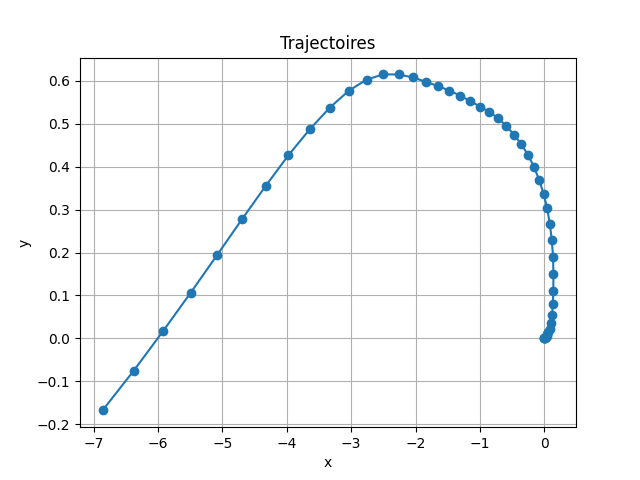
\includegraphics[width=.5\textwidth]{images/SINGER_Trajectoire_1.png} 
  Paramètres : $T_{ech} = 1$, $N = 50$, $\sigma^{2} = \frac{2}{3}.10^{-6}$ et $\alpha = \frac{1}{30}$
\end{frame}

\begin{frame}
  \frametitle{Trajectoires : Singer}
  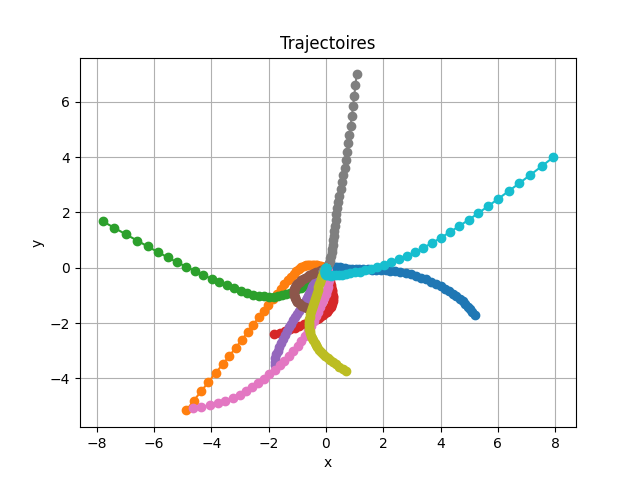
\includegraphics[width=0.75\textwidth]{images/SINGER_Trajectoires.png}
  Paramètres : $T_{ech} = 1$, $N = 50$, $\sigma^{2} = \frac{2}{3}.10^{-6}$ et $\alpha = \frac{1}{30}$
\end{frame}

% Récapitulatif des Trajectoires
\begin{frame}
    \frametitle{Récapitulatif des Trajectoires}
    \begin{figure}
    \centering
    \begin{minipage}{0.3\textwidth}
        \centering
        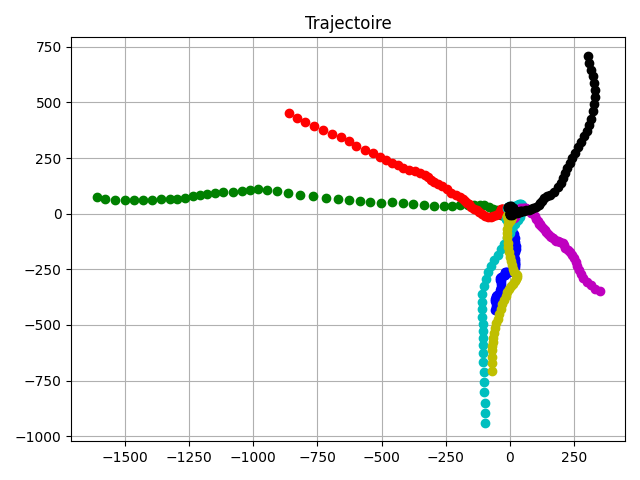
\includegraphics[width=\textwidth]{images/MRU_Trajectoires.png}
        \caption{MRU}
    \end{minipage}
    \begin{minipage}{0.3\textwidth}
        \centering
        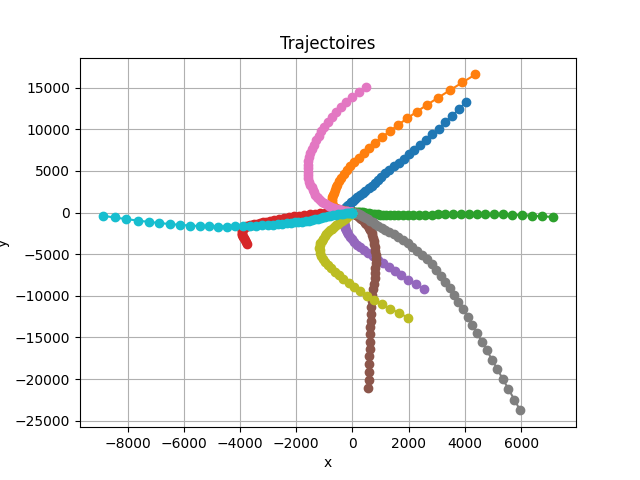
\includegraphics[width=\textwidth]{images/MUA_Trajectoires.png}
        \caption{MUA}
    \end{minipage}
    \begin{minipage}{0.3\textwidth}
        \centering
        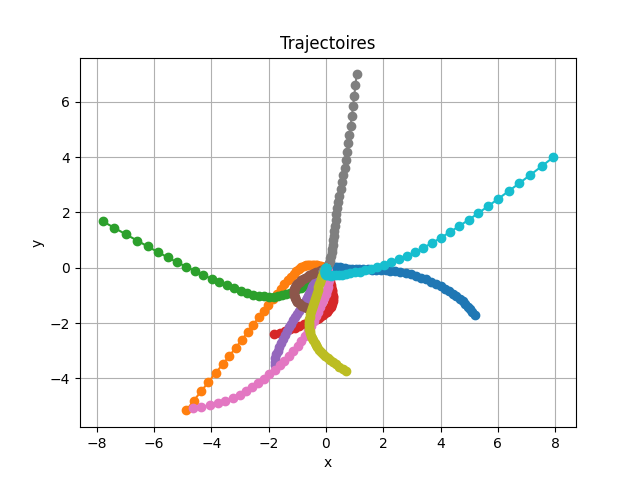
\includegraphics[width=\textwidth]{images/SINGER_Trajectoires.png}
        \caption{SINGER}
    \end{minipage}
\end{figure}
\end{frame}

% Présentation des méthodes et outils de travail
\begin{frame}
    \frametitle{Méthodes et Outils de Travail}
    \begin{itemize}
        \item \textbf{\href{https://github.com/Feulym/ProjetS8_TRACK_2425}{GitHub}} : Répertoire général avec tous les codes (Python et Latex) et les images pour les CR
        \item \textbf{\href{https://trello.com/b/AcVzNkta/projet-s8-track}{Trello}} : Pour le suivi des tâches à faire/en cours/terminée et le suivi de l'avancement (lien d'invitation : \href{https://trello.com/invite/b/67936f0df0a78c335e0e61e9/ATTIa74f84297b27934504d49c129702a97d20B0A929/projet-s8-track}{ici})
        \item \textbf{Canal Télégram} : canal d'échange et de discussion
    \end{itemize}
\end{frame}

% Trello
\begin{frame}{Organisation avec Trello}

  \begin{figure}
      \centering
      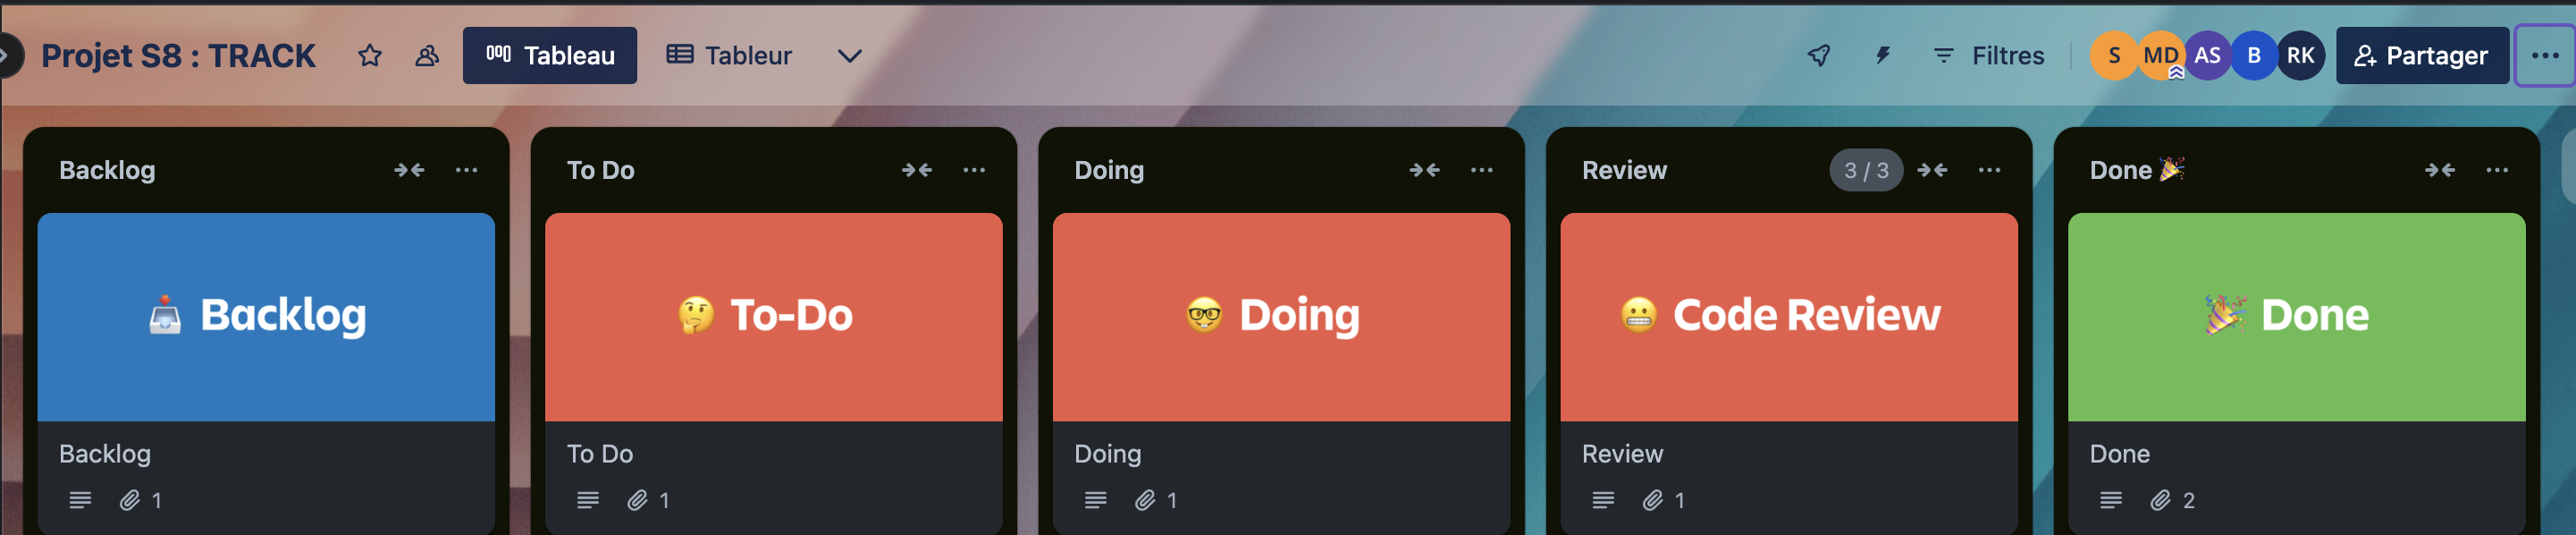
\includegraphics[width=1\linewidth]{images/trello}
      \caption{Capture d'écran de notre espace Trello}
      \label{fig:trello}
  \end{figure}
  
  \begin{itemize}
      \item Division du travail à réaliser en plusieurs tâches grâce à un tableau Kanban, pour assurer un meilleur suivi global.
      \item Organisation du travail selon plusieurs sprints.
  \end{itemize}
  
\end{frame}

% Calendrier de travail
\begin{frame}
  \frametitle{Calendrier de travail}
    \begin{itemize}
        \item Pour la semaine prochaine : 
        \begin{itemize}
            \item[\hspace{1cm}] Générer les bases de données 
            \item[\hspace{2cm}] ($\sim$ 50,000 échantillons | tailles variables ($100 < N < 750$))
        \end{itemize}
        \item La suite ?
    \end{itemize}
\end{frame}

% Questions
\begin{frame}
  \frametitle{Questions}
  \begin{itemize}
    \item Cohérence des courbes ?
    \item Quelle quantité d'échantillons ? Tailles variables des échantillons ?
    \item Rebruiter nos données générées ? 
    \item Un format de stockages de donnés à privilégier ?
  \end{itemize}
\end{frame}

% Fin de la présentation
\end{document}
